\chapter{Implementation}

In this chapter, we will introduce the implementation details of our method. The difference between this chapter and the previous one is that the concepts introduced in the method chapter are easily adaptable to any kind of implementation environment, while in this chapter we focus on a GPU-oriented implementation. First, we will give a general outline of our algorithm. Then, we will take each one of the single parts of the algorithm and discuss them separately. After introducing the details of the algorithm, we will discuss some caveats that are necessary in order to eliminate defects and artifacts in our algorithm. Finally, we will discuss our implementation, introducing some possible implementation alternatives in order to compare them in the result section.

\section{Environment}

In order to better contextualize some of the choices and the code parts that will be introduced in this section, we will first introduced the environment used in our implementation. The method we are going to discuss was made using the OpenGL API, version 4.3 (released in August 2012), a multi-platform API used for rendering 2D and 3D accelerated graphics. With the OpenGL API comes together GLSL, the OpenGL Shading Language, used for writing pieces of code to be run on the GPU, called \emph{shaders}. Our method uses some advanced features of OpenGL 4.3, so it is not immediately portable to previous generation hardware, and runs only on high-end modern GPUs. On the CPU side, we use an extended framework based on Qt, a C++ library that allows to create OpenGL contexts and graphical interfaces in an easy way.


Stuff to insert:
\begin{itemize}
	\item Generation of random points
	\item Noise generation on GPU
	\item Sampling patterns
	\item Layered rendering
	\item Shadow mapping (for lights)
	\item Ping-ponging and accumulation
	\item Texture Views and mipmap generation (memory optimization)
	\item Engine structure
	\item Extension: compute shaders
	\item Extension: image load store (meh)
	\item Extension: cubemap
	\item Extension: subroutines (meh)
	\item Sampling colormap
	\item Alternative: voxelization

\end{itemize}

Caveats:
\begin{itemize}
	\item Oversampling issues in final combinaiton (multisampling of depth map)
	\item Combination delta
	\item Shadow bias
  \item Random rotation
	
\end{itemize}

\begin{lstlisting}[language=GLSL,label=test,caption=Test!]
#version 430
layout(triangles) in;
layout(triangle_strip, max_vertices = 60) out;

#include "ss_aincludes_constants.glinc"

uniform int layers;
uniform mat4 P;
uniform mat4 viewMatrices[DIRECTIONS];

smooth in vec3 v_position[3];
smooth in vec3 v_norm[3];

smooth out vec3 position;
smooth out vec3 norm;

void main(void)
{
    int l = layers;
    for(int i = 0; i < l; i++)
    {
        gl_Layer = i;

        for(int k = 0; k < 3; k++)
        {
            vec4 v0 = gl_in[k].gl_Position;
            position = v_position[k];
            norm = v_norm[k];
            gl_Position = P * viewMatrices[i] * v0;
            EmitVertex();
        }

        EndPrimitive();
    }
}
\end{lstlisting}

In this chapter, we describe the implementation details of our technique, using the approximation of the rendering equation introduced in the previous chapter. We start by giving a rather generic introduction of our algorithm, introducing then all the implementation details. 


%\section{Requirements}
%
%Our algorithm, in order to be generic and applicable to a wide range of situations must meet some requirements. 
%
%
%\begin{itemize}
  %\item The algorithm should be \emph{accurate}, so that the renderings are as close as possible to reference images generated using a offline Monte-Carlo simulation. 
	%\item The algorithm should be \emph{fast}, executing at interactive frame rates.
	%\item The algorithm should be \emph{uv-independent}, not relying on a pre-made UV mapping of the object in order to being able to perform. The algorithm should work only if basic geometric features are provided (vertices and normals).
	%\item The algorithm should be \emph{adaptable}, handling in real-time dynamic light changes and object deformations. So it will not possible to use light baking or geometry form factors.
%\end{itemize}
%
%If it is not possible to satisfy all the previous within the strict constraints of real-time rendering, we want to create an algorithm that gets as close as possible to the requested result. The algorithm should progressively progressively improve and converge to an accurate result whenever possible (e.g. when the light in the scene is not changing).

\section{Algorithm overview}

By keeping the limitations presented in the previous chapter in mind TODO, we introduce our four pass algorithm. The algorithm is inspired by \emph{translucent shadow maps} TODO, that we presented in chapter TODO. The general idea is to first render the scene from the light point of view, then place the disk we discussed in the method chapter TODO directly on the generated texture. We use many directions in order to capture all the sides of the object. In this section, we will assume to only have one directional light $L_d$, $\vomega_d$ and one not-deformable object in the scene. We will discuss later how to extend the method to multiple light sources.

\textbf{Step 1 - Light buffer} \\

In the first step, positions and normals of the object are rendered into a texture from the light point of view. As in standard shadow mapping we create and store a matrix to convert between world space and texture light space. With the matrix definitions and notation in section \ref{sec:matrices}, we express the matrix as:

$$
L = T\left(\frac{1}{2}\right) \cdot S\left(\frac{1}{2}\right) \cdot P \cdot V
$$

where $P$ and $V$ are the projection and view matrix we use to render with the light. The first two matrices are necessary to convert between clip and texture coordinates, as clip coordinates are in the range $[-1,1] \times [-1,1]$, while texture coordinates are in the range $[0,1]\times[0,1]$. 

\begin{figure}[!ht]
\centering
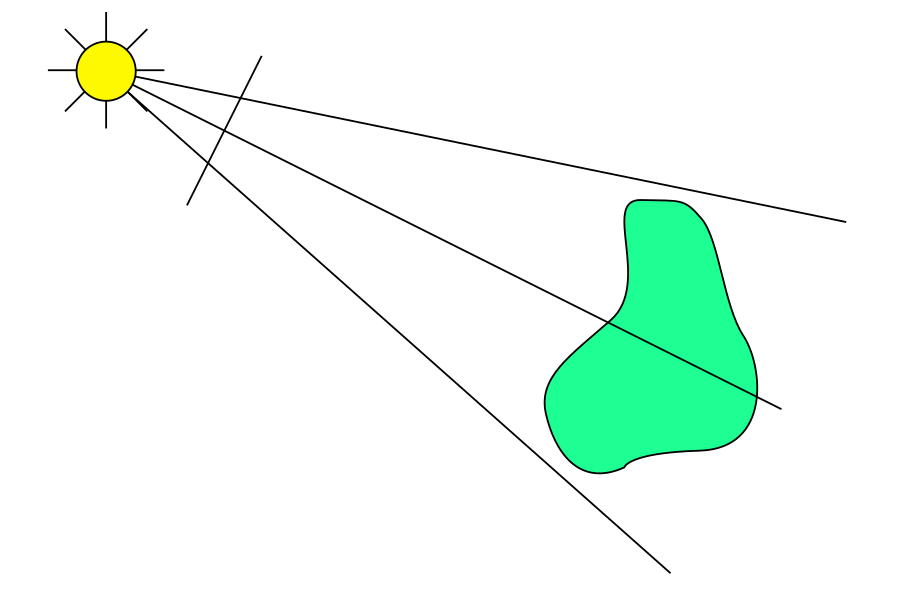
\includegraphics[width=0.8 \linewidth]{images/method/step1.pdf}
\caption{Render to G-buffer. Note that the frustum and the light direction are aligned.}
\label{fig:step1}
\end{figure} 


\begin{figure}
\centering
\subfloat[{Vertex buffer}]{
  \includegraphics[width=0.5 \linewidth]{images/method/vertices.png}
  \label{fig:vbuff}
}
\subfloat[{Normal buffer}]{
  \includegraphics[width=0.5 \linewidth]{images/method/normals.png}
  \label{fig:nbuff}
} 
\label{fig:lightbuffers}
\caption{State of the vertex and normal buffer after rendering from a directional light. The model used was the Stanford bunny from the Standford 3D Scanning repository.}
\end{figure}

\FloatBarrier

\textbf{Step 2 - Render to radiance map} \\
In the second step, we render the object from $K$ different directions into a radiance map. The radiance map is organized as a layered texture, where each layer represents a direction. The points on which to place the cameras are chosen randomly. On each layer, we accumulate the result over different frames. On the rendering step, for each pixel that corresponds to an exitance point $\x_o$ the shader samples $N$ points from the texture rendered in the previous step. If the sampled point is valid, it is then used to calculate the BSSRDF and accumulate it in the resulting radiance map. So, this step calculates the following:

$$
R^{t,k}(\x_o) = L_d \sum_{i = 1}^N S(\x^{t,k}_i, \vomega^t_l, \x_o, \vomega_o) \exp\left(\sigma_{tr} r^{t,k}_i\right), \ \ t \in [0,T], \ \ k \in [0,K-1] 
\label{eq:evolution_step}
$$

\begin{figure}[!ht]
\centering
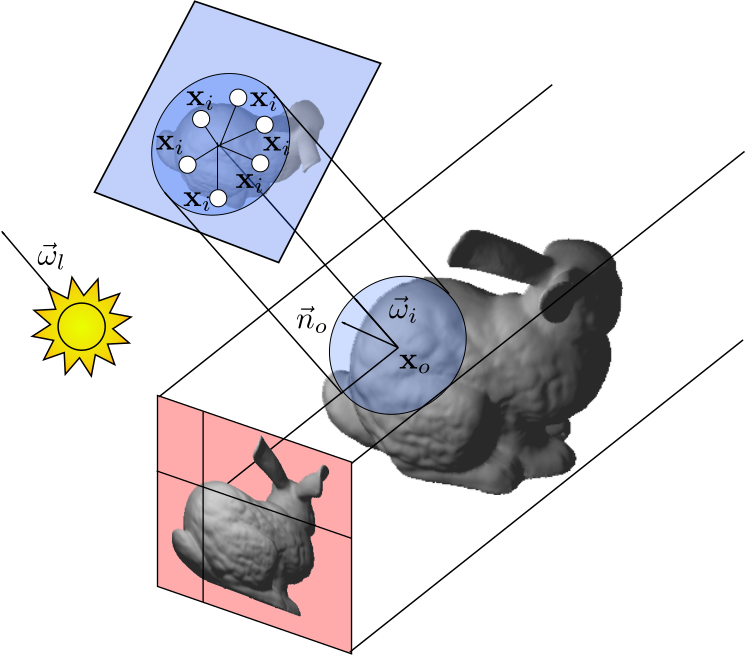
\includegraphics[width=0.9 \linewidth]{images/method/step2_improved.pdf}
\caption{Render to the radiance map. When we render the point $\x_o$, the position in the lightmap is calculated and the values $\x_i$ in the samples are calculated and summed over.}
\label{fig:step2}
\end{figure} 

Where we recall that we have introduced an exponential term in order to compensate for the exponential displacement of the sampling pattern. We introduced also a time $t$ parameter, that represents the fact that the result change over time, and a $k$ parameter, that represents the current direction we are rendering to. We will come back to this accumulation concept in a few lines. We can see how we are rendering a point from one of the considered directions in Figure \ref{fig:stepfrustum}. Also in this case, the texture space - world space conversion matrices are stored and prepared to be reused in the final combination step. 

We can appreciate that rendering the light from the camera point of view comes with two important advantages:

\begin{itemize}
	\item If the disk is placed in texture space, it is automatically oriented towards the light direction, that is $\vomega_d = \vomega_l$.
	\item The light renders in the texture only the points directly visible from it, that are also the points where the light radiance is maximum. In addition, if we sample the lightmap on any point, we get the corresponding vertex that is closest to the light.
\end{itemize}

This two factors allows us to sample the most optimal point and direction in where to place the disk, as we described it in section TODO.
 
\begin{figure}[!ht]
\centering
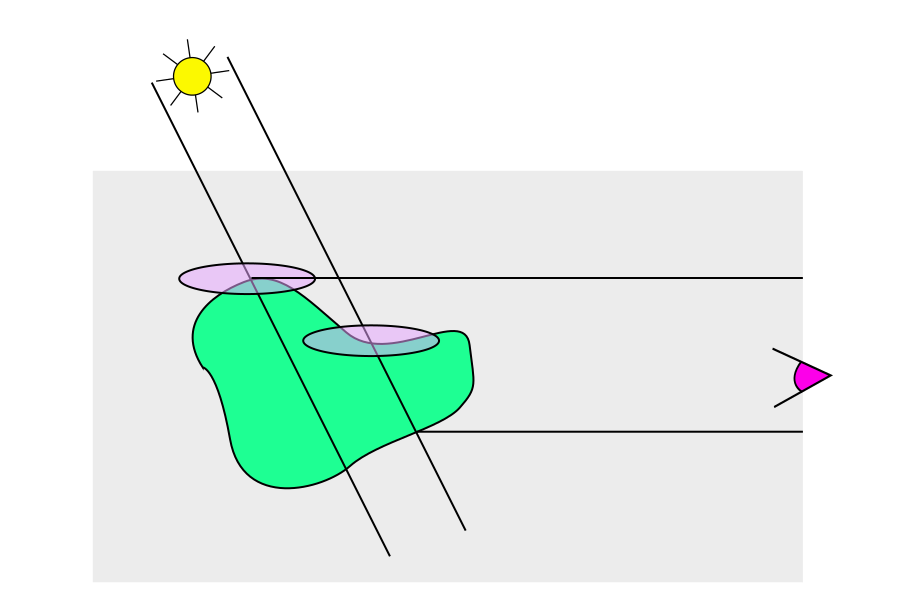
\includegraphics[width=\linewidth]{images/method/step2}
\caption{Render to cubemap, side view. The gray area represents the frustum of the current direction's camera (orthographic). We have three different cases of a point on the surface: $\x_o^1$ is visible from both the light and the camera, so the disk is placed on it. $\x_o^2$ is visible from the camera but not from the light, so the disk is placed in the closest position to the light. $\x_o^3$ is not visible from the camera, so it is discarded.}
\label{fig:stepfrustum}
\end{figure} 

As we discussed, these is an accumulation process going on:

$$
\tilde{R}^{t,k} = \sum_{i = 0}^{t-1} R^{i,k} + R^{t,k} = \tilde{R}^{t-1, k} + R^{t,k}
$$

$\tilde{R}$ here represents the actual value that is stored in the texture or loaded from the previous one. Naturally, the accumulation process works only if the scene does not change. A change can be a relative change of positions between the points on the model and the light, so if the model gets rotated or scaled (translation for directional lights is irrelevant), the accumulated result has to be discarded and the accumulation started all over. The cameras are locked with the model, so the pixels are always aligned irregardless of the model matrix of the object. This is why in equation \ref{eq:evolution_step} the dependence from time of the point $\x_o$ and $\vomega_o$ have been dropped. Obviously, the dependence must be reintroduced in case we are dealing with deformable objects.
 
\FloatBarrier

\textbf{Step 3 - Combination} \\
In this step, we have the final render of our model. While all the previous steps were not rendering anything in the scene (making a render-to-texture), in this scene we do an actual rendering of the model. Using the matrices prepared in the previous step, for each fragment on the surface we sample all the layers in the texture as illustrated in Figure \ref{fig:step3}. In order to do this, we need also to sample the depth map generated in the previous step. We can define this sampling as a visibility function to test if a point $\x$ belongs to layer $k$:

$$
V_i^k(\x) = \begin{cases}
1 & \text{if $\x$ is visible from the $k$th camera} \\
0 & \text{otherwise}
\end{cases}
$$
Given this function, we can simply represent the outgoing radiance by simply averaging the summation over the $K$ layers:

$$
L_{SS}^t(\mathbf{x}) = \frac{A_c}{N (t + 1)} \frac{\displaystyle\sum_{k = 0}^{K-1}V_{i}^k(\x) \tilde{R}^{t,k}(\mathbf{x})}{\displaystyle\sum_{k = 0}^{K-1}V_{i}^k(\x)}
$$

The first factor $\frac{1}{t + 1}$ is to average over the number of frames, while the second is the average area of a sample in the circle $\frac{A_c}{N}$, that is necessary to complete the equation as described in TODO. We note that we tried to move all the layer-independent computation into the final computation step, in order to save as much performance as possible. 

\begin{figure}[!ht]
\centering
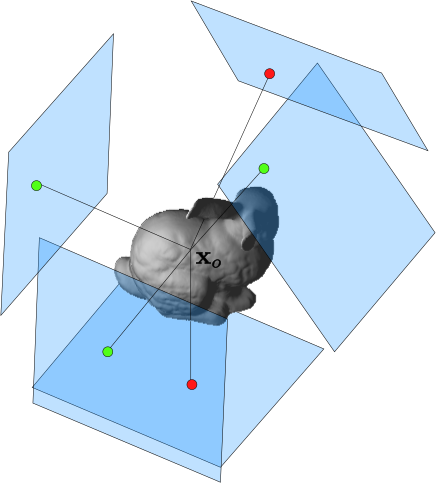
\includegraphics[width=0.8 \linewidth]{images/method/combination.pdf}
\caption{Final combination step. The blue quads indicates each one of the radiance map layers, as seen from their direction. We can see that in the point $\x_o$ the contribution from three faces (green dots) is considered. For the remaining two faces (red dots), the contribution is not considered as the point is not visible.}
\label{fig:step3}
\end{figure} 

We are not done yet, as for now we have computed the radiance only deriving from subsurface scattering. For finally describing the illumination of our scene, we need also to include a factor based on the surface reflection. Since the subsurface scattering radiance is already multiplied by a transmittance Fresnel term (in the BSSRDF equation in TODO) $T(\eta,\vomega_o)$ we the reflection color multiplied by the converse transmission term $1 - T(\eta,\vomega_o)$:

$$
L^t(\x, \vomega_o) = L_{SS}^t(\x) + (1 - T(\eta,\vomega_o)) L_i(\x, \vomega_o - 2 (\vomega_o \cdot \vec{n}) \vec{n})
$$

$L_i$ can be the radiance coming from other objects or by an environment map. After this, we just need to perform gamma correction in order to get the final result. Given the gamma coefficient $\gamma$, we perform gamma correction by:

$$
L_{gamma}^t(\x, \vomega_o, \gamma) = L^t(\x,\vomega_o)^{\frac{1}{\gamma}}
$$

And we can finally send the radiance to the output device.


\clearpage
\section{Implementation details}

\section{Artifacts}
A simple implementation of the method described until now is not completely correct. In fact, since we are discretizing the surface on a texture, some sampling artifacts are inevitable. During our implementation we identified three different types of artifacts:

\begin{itemize}
	\item Incorrect sampling of the G-buffer
	\item Incorrect sampling of the cubemap
	\item Shadow bias (when sampling the depth of the texture).
\end{itemize}

That are described in detail in the following sections.

\subsection{Incorrect sampling of the G-buffer}

In order to sample the G-buffer correctly, we need to modify the world coordinate of the point $\mathbf{x}_o$ with normal $\vec{n}_o$ in order to "shrink" a little bit towards the inside of the object according to the light direction $\vec{\omega}_l$:

$$
\mathbf{x}_o' = \mathbf{x}_o - \epsilon_g (\vec{n}_o - \vec{\omega}_l ( \vec{\omega}_l \cdot  \vec{n}_o))
$$

\subsection{Incorrect sampling of the cubemap}

Since we are sampling a cubemap, we do not need to account for the light direction in this case. In addition, the cubemap needs a 3D vector to be sampled with. So, instead of using $\mathbf{x}_o$, we use a point slightly intruded (i.e. displaced along the normal) in the calculations, according to:

$$
\mathbf{x}_o' = \mathbf{x}_o - \epsilon_c \vec{n}_o
$$

\subsection{Shadow bias}

In order to avoid artifacts such as shadows acne, we use a bias when comparing the z values of a point to determine if the point is in shadow or not. This implies that we need to convert the depth value from texture space ($\mathbf{z}_{tex}$) to world space again ($\mathbf{z}_{world}$). Since we are using an orthographics camera, the z value is the same in clip coordinates and in normalized device coordinates. Then, we simply use the camera projection properties ($\mathbf{z}_{far}$, $\mathbf{z}_{near}$) to convert the depth into the camera local space, in order to finally add the camera position transformed z value ($\mathbf{z}_{camera}$) and reconstruct the depth in world space:

$$
\mathbf{z}_{world} = \mathbf{z}_{camera} - \frac{\mathbf{z}_{far} - \mathbf{z}_{near}}{2} \left( 2 \mathbf{z}_{tex} - 1 + \frac{\mathbf{z}_{far} + \mathbf{z}_{near}}{\mathbf{z}_{far} - \mathbf{z}_{near}}\right)
$$
		
And finally compare the obtained z with the z position in world space of the point ($\mathbf{z}$) using the bias $\epsilon_b$, so a point is lit iff:

$$
\mathbf{z}_{world} - \epsilon_b < \mathbf{z}
$$		

\begin{figure}
\centering
\subfloat[Without shadow bias and sampling fixes]{
  \includegraphics[width=0.45 \linewidth]{images/artifacts/all}
  \label{fig:art_ss1}
} 
\subfloat[With shadow bias and without sampling fixes]{
  \includegraphics[width=0.45 \linewidth]{images/artifacts/nobias}
  \label{fig:art_ss2}
} 
\\
\subfloat[With both shadow bias and sampling fixes]{
  \includegraphics[width=0.45 \linewidth]{images/artifacts/cmboffset}
  \label{fig:art_ss3}
}
\subfloat[Reference]{
  \includegraphics[width=0.45 \linewidth]{images/artifacts/reference}
  \label{fig:art_ss4}
}
\caption{Progressively removing artifacts to get to the final image. }
\label{fig:artifacts}
\end{figure} 
